% vim: set tw=78 sts=2 sw=2 ts=8 aw et:
\documentclass{so.cs.pub.ro}

\usepackage{code/highlight}

\title[Laborator 8]{Laborator 8}
\subtitle{Thread-uri}

\begin{document}

\frame{\titlepage}

% Titlul unui frame se specifică fie în acolade, imediat după \begin{frame},
% fie folosind \frametitle

\begin{frame}{Thread Control Block}
\begin{columns}

\begin{column}[1]{0.38\textwidth}
	\begin{itemize}
		\item Informații partajate
   	\begin{itemize}
    		\item Spațiu de adresă
   		\item Heap, Data
   		\item Semnale și handlere
   		\item I/O și fișiere
  	 	\end{itemize}
   	\item Informații proprii
   	\begin{itemize}
   		\item Starea
   		\item Regiștrii
   		\item Program counter
   		\item Stiva
   		\item Masca de semnale
   		\item errno
   	\end{itemize}
	\end{itemize}
\end{column}
\begin{column}[1]{0.52\textwidth}
\framebox{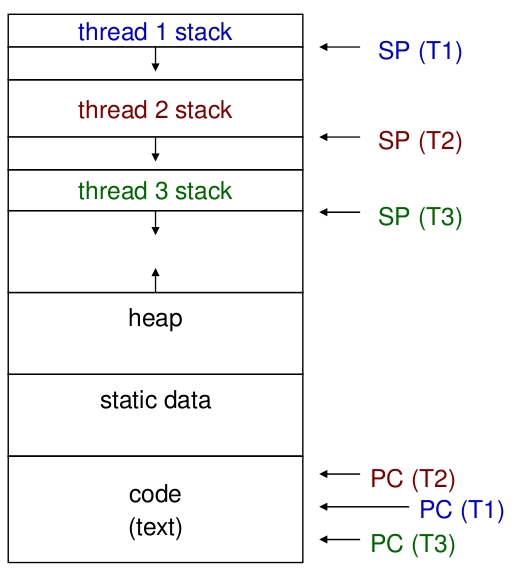
\includegraphics[width=2.5in]{code/tas.jpg}}
\end{column}
\end{columns}
\end{frame}

\begin{frame}{Avantaje}
\begin{itemize}
	\item Pot comunica între ele fără a implica kernelul
	\item Asigură o folosire mai eficientă a resurselor calculatorului
	\item Mai puțin timp pentru crearea/distrugerea unui thread decât a unui proces
	\item Comutarea între 2 thread-uri mai rapidă decât între procese
	\vspace{0.3cm}
	\item Paralelizarea are sens in 2 situații:
	\begin{itemize}
		\item Task-uri I/O bound pe același CPU
		\item Task-uri CPU bound pe mai multe core-uri
	\end{itemize}
	\vspace{0.3cm}
	\item dezavantaj: sincronizare (overhead + model de programare complex)
\end{itemize}
\end{frame}

\begin{frame}{Thread-uri – noțiuni generale}
\begin{itemize}
	\item Nu întotdeauna dorim să partajăm totul cu celelalte thread-uri $=>$ e nevoie de un storage thread-specific
	\vspace{0.1cm}
	\item O zonă din stiva fiecărui thread este organizată sub forma unui Map cu perechi (cheie, valoare)
	\vspace{0.1cm}
	\item Atenție la crearea de foarte multe thread-uri cu stivă mare (se poate epuiza spațiul de adrese)
	\vspace{0.5cm}
	\item Există 3 tipuri de implementări : ULT, KLT, hibride
\end{itemize}
\end{frame}

\begin{frame}{ULT vs. KLT}
\begin{itemize}
	\item {\bf User-Level Threads}
	\begin{itemize}
		\item Kernel-ul nu este conștient de existenţa lor
		\item Schimbarea de context nu implică kernelul $=>$ rapidă
		\item Planificarea poate fi aleasă de aplicaţie
		\item Aceste thread-uri pot rula pe orice SO
		\item Dacă un thread apelează ceva blocant toate thread-urile planificate de aplicaţie vor fi blocate
		\item 2 fire ale unui proces nu pot rula simultan pe 2 procesoare
	\end{itemize}
	\vspace{0.1cm}
	\item {\bf Kernel-Level Threads}
	\begin{itemize}
		\item Schimbarea de context între thread-uri ale aceluiași proces implică kernel-ul
		$=>$ viteza de comutare este mică
		\item Blocarea unui fir nu înseamnă blocarea întregului proces
		\item Dacă avem mai multe procesoare putem lansa în execuţie simultană mai multe thread-uri ale aceluiași proces
	\end{itemize}
\end{itemize}
\end{frame}

\begin{frame}{Thread Safety / Reentranță}
	\begin{itemize}
		\item {\bf Thread-safe} - Operații sigure în context multithreading
		\begin{itemize}
		\item o funcție este thread-safe dacă și numai dacă va produce mereu rezultatul corect atunci când este apelată concurent, în mod repetat, din mai multe thread-uri
   	\end{itemize}
   	\vspace{0.3cm}
		\item Tipuri de funcții thread-unsafe
		\begin{itemize}
   		\item Funcții ce nu protejează variabilele partajate
   		\item Funcții ce întorc pointer la o variabilă statică
   		\item Funcții ce apelează funcții thread-unsafe
   	\end{itemize}
   	\vspace{0.3cm}
   	\item Funcțiile {\bf reentrante} sunt cele care nu referă date partajate
		\begin{itemize}
			\item nu lucrează cu variabile globale/statice
   		\item nu apelează funcții non-reentrante
   		\item sunt un subset al funcțiilor thread-safe
	  	\end{itemize}
   	\vspace{0.1cm}
   	\item un apel reentrant în execuție nu afectează un alt apel simultan
   \end{itemize}
\end{frame}


\begin{frame}{Mecanisme de sincronizare}
	\begin{itemize}    % Just like normal LaTeX
		\item Mutex (POSIX, Win32)
		\item Semafor (POSIX, Win32)
		\item Secţiune critică (Win32)
		\item Variabilă de condiţie (POSIX, Win32)
		\item Barieră (POSIX, Win32)
		\item Operaţii atomice cu variabile partajate (Win32)
		\item Thread pooling (Win32)
	\end{itemize}
\end{frame}



%\begin{frame}{Întrebări}
%\begin{itemize}
%\item Cum se modifică spațiul de adresă al unui proces la schimbarea de context între două fire de execuție?
%\item Un proces are 4 fire de execuție. Unul din firele de execuție, face un access invalid la memorie. Ce se întâmplă
%cu celelalte 3 fire de execuție?
%\item Descrieți o situație în care folosirea firelor de execuție ar duce la degradarea performanței?
%\item Descrieți o situție (pe un sistem uniprocesor) în care folosind fire de execuție îmbunătățim performanța unui
%program.
%\end{itemize}
%\end{frame}

\end{document}
